\documentclass{standalone}
\usepackage{tikz}
\usetikzlibrary{patterns, positioning}


\begin{document}
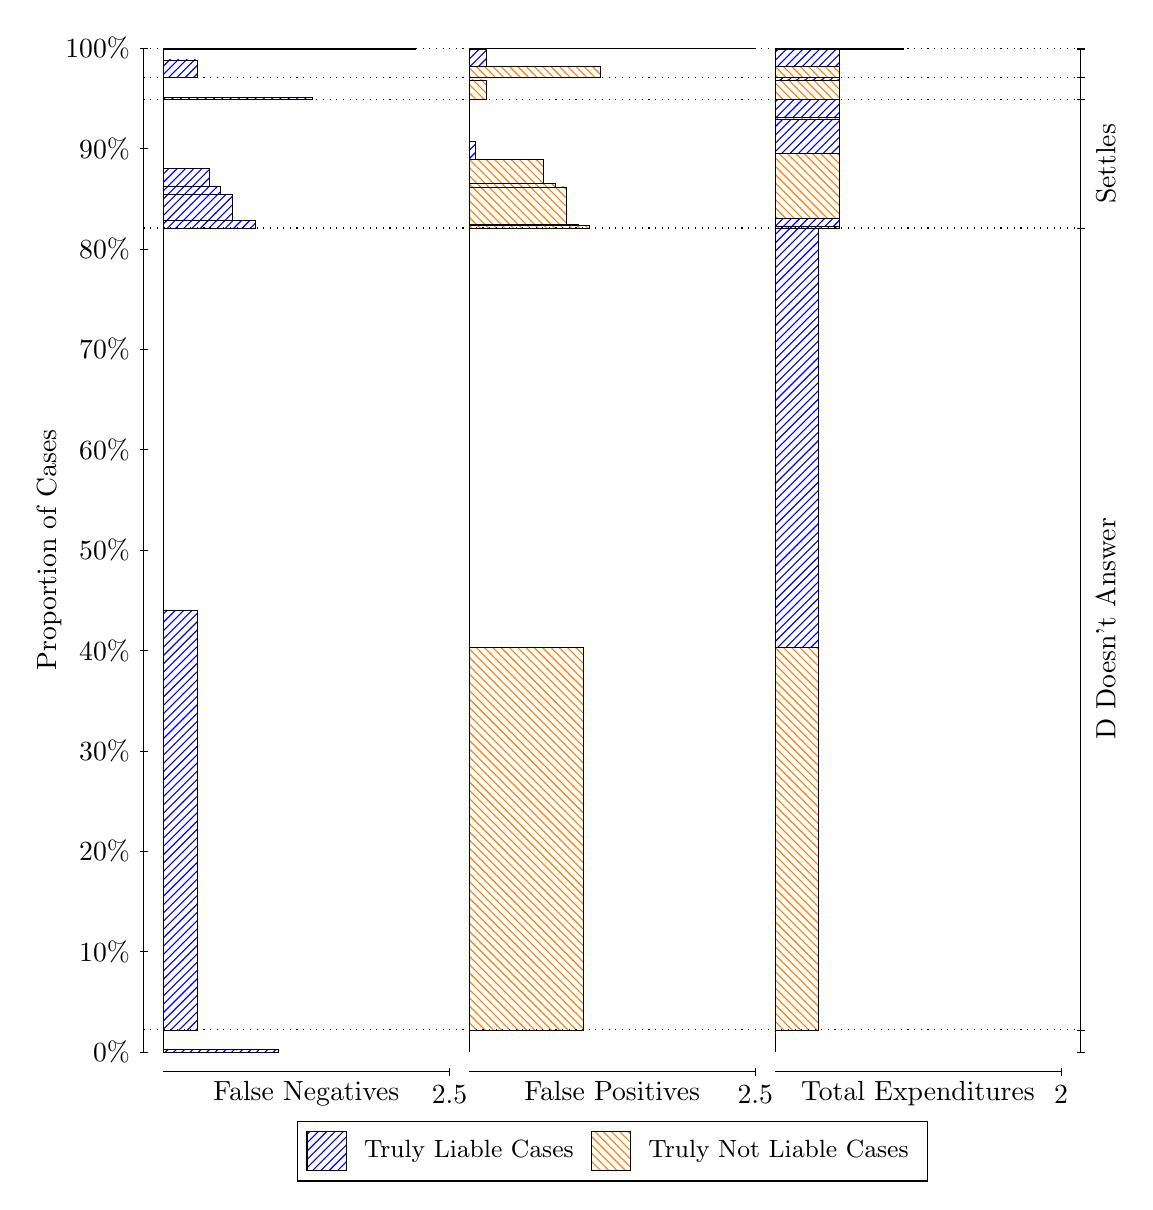
\begin{tikzpicture}
\draw[black, very thin] (1.5,1.75) -- (1.5,14.5);
\node[rotate=90, text=black, anchor=center] at (0.3, 8.125) {Proportion of Cases};
\draw[black, very thin] (1.45,1.75) -- (1.55,1.75);
\node[text=black, anchor=east] at (1.45, 1.75) {0\%};
\draw[black, very thin] (1.45,3.025) -- (1.55,3.025);
\node[text=black, anchor=east] at (1.45, 3.025) {10\%};
\draw[black, very thin] (1.45,4.3) -- (1.55,4.3);
\node[text=black, anchor=east] at (1.45, 4.3) {20\%};
\draw[black, very thin] (1.45,5.575) -- (1.55,5.575);
\node[text=black, anchor=east] at (1.45, 5.575) {30\%};
\draw[black, very thin] (1.45,6.85) -- (1.55,6.85);
\node[text=black, anchor=east] at (1.45, 6.85) {40\%};
\draw[black, very thin] (1.45,8.125) -- (1.55,8.125);
\node[text=black, anchor=east] at (1.45, 8.125) {50\%};
\draw[black, very thin] (1.45,9.4) -- (1.55,9.4);
\node[text=black, anchor=east] at (1.45, 9.4) {60\%};
\draw[black, very thin] (1.45,10.675) -- (1.55,10.675);
\node[text=black, anchor=east] at (1.45, 10.675) {70\%};
\draw[black, very thin] (1.45,11.95) -- (1.55,11.95);
\node[text=black, anchor=east] at (1.45, 11.95) {80\%};
\draw[black, very thin] (1.45,13.225) -- (1.55,13.225);
\node[text=black, anchor=east] at (1.45, 13.225) {90\%};
\draw[black, very thin] (1.45,14.5) -- (1.55,14.5);
\node[text=black, anchor=east] at (1.45, 14.5) {100\%};

\draw[black, very thin] (13.4,1.75) -- (13.4,14.5);
\draw[black, very thin] (13.35,1.75) -- (13.45,1.75);
\node[anchor=west] at (13.35, 1.75) {};
\draw[black, very thin] (13.35,2.0298) -- (13.45,2.0298);
\node[anchor=west] at (13.35, 2.0298) {};
\draw[black, very thin] (13.35,12.215) -- (13.45,12.215);
\node[anchor=west] at (13.35, 12.215) {};
\draw[black, very thin] (13.35,13.844) -- (13.45,13.844);
\node[anchor=west] at (13.35, 13.844) {};
\draw[black, very thin] (13.35,14.126) -- (13.45,14.126);
\node[anchor=west] at (13.35, 14.126) {};
\draw[black, very thin] (13.35,14.489) -- (13.45,14.489);
\node[anchor=west] at (13.35, 14.489) {};
\draw[black, very thin] (13.35,14.496) -- (13.45,14.496);
\node[anchor=west] at (13.35, 14.496) {};
\draw[black, very thin] (13.35,14.5) -- (13.45,14.5);
\node[anchor=west] at (13.35, 14.5) {};

\draw[black, very thin, pattern color=blue, pattern=north east lines] (1.75,1.75) rectangle (3.2033,1.7794);
\draw[black, very thin, pattern color=orange, pattern=north west lines] (1.75,1.7794) rectangle (1.75,2.0298);
\draw[black, very thin, pattern color=blue, pattern=north east lines] (1.75,2.0298) rectangle (2.186,7.3589);
\draw[black, very thin, pattern color=orange, pattern=north west lines] (1.75,7.3589) rectangle (1.75,12.215);
\draw[black, very thin, pattern color=blue, pattern=north east lines] (1.75,12.215) rectangle (2.9127,12.31);
\draw[black, very thin, pattern color=blue, pattern=north east lines] (1.75,12.31) rectangle (2.7673,12.314);
\draw[black, very thin, pattern color=blue, pattern=north east lines] (1.75,12.314) rectangle (2.622,12.644);
\draw[black, very thin, pattern color=blue, pattern=north east lines] (1.75,12.644) rectangle (2.4767,12.746);
\draw[black, very thin, pattern color=blue, pattern=north east lines] (1.75,12.746) rectangle (2.3313,12.973);
\draw[black, very thin, pattern color=orange, pattern=north west lines] (1.75,12.973) rectangle (1.75,13.844);
\draw[black, very thin, pattern color=blue, pattern=north east lines] (1.75,13.844) rectangle (3.6393,13.875);
\draw[black, very thin, pattern color=orange, pattern=north west lines] (1.75,13.875) rectangle (1.75,14.126);
\draw[black, very thin, pattern color=blue, pattern=north east lines] (1.75,14.126) rectangle (2.186,14.349);
\draw[black, very thin, pattern color=orange, pattern=north west lines] (1.75,14.349) rectangle (1.75,14.489);
\draw[black, very thin, pattern color=blue, pattern=north east lines] (1.75,14.489) rectangle (4.9473,14.491);
\draw[black, very thin, pattern color=orange, pattern=north west lines] (1.75,14.491) rectangle (1.75,14.496);
\draw[black, very thin, pattern color=orange, pattern=north west lines] (1.75,14.496) rectangle (1.75,14.498);
\draw[black, very thin, pattern color=blue, pattern=north east lines] (1.75,14.498) rectangle (1.75,14.5);
\draw[black, very thin, pattern color=orange, pattern=north west lines] (5.6333,1.75) rectangle (5.6333,2.0004);
\draw[black, very thin, pattern color=blue, pattern=north east lines] (5.6333,2.0004) rectangle (5.6333,2.0298);
\draw[black, very thin, pattern color=orange, pattern=north west lines] (5.6333,2.0298) rectangle (7.0867,6.8859);
\draw[black, very thin, pattern color=blue, pattern=north east lines] (5.6333,6.8859) rectangle (5.6333,12.215);
\draw[black, very thin, pattern color=orange, pattern=north west lines] (5.6333,12.215) rectangle (7.1593,12.243);
\draw[black, very thin, pattern color=orange, pattern=north west lines] (5.6333,12.243) rectangle (7.014,12.259);
\draw[black, very thin, pattern color=orange, pattern=north west lines] (5.6333,12.259) rectangle (6.8687,12.737);
\draw[black, very thin, pattern color=orange, pattern=north west lines] (5.6333,12.737) rectangle (6.7233,12.78);
\draw[black, very thin, pattern color=orange, pattern=north west lines] (5.6333,12.78) rectangle (6.578,13.086);
\draw[black, very thin, pattern color=blue, pattern=north east lines] (5.6333,13.086) rectangle (5.706,13.313);
\draw[black, very thin, pattern color=blue, pattern=north east lines] (5.6333,13.313) rectangle (5.6333,13.844);
\draw[black, very thin, pattern color=orange, pattern=north west lines] (5.6333,13.844) rectangle (5.8513,14.094);
\draw[black, very thin, pattern color=blue, pattern=north east lines] (5.6333,14.094) rectangle (5.6333,14.126);
\draw[black, very thin, pattern color=orange, pattern=north west lines] (5.6333,14.126) rectangle (7.3047,14.266);
\draw[black, very thin, pattern color=blue, pattern=north east lines] (5.6333,14.266) rectangle (5.8513,14.489);
\draw[black, very thin, pattern color=orange, pattern=north west lines] (5.6333,14.489) rectangle (5.6333,14.494);
\draw[black, very thin, pattern color=blue, pattern=north east lines] (5.6333,14.494) rectangle (5.6333,14.496);
\draw[black, very thin, pattern color=orange, pattern=north west lines] (5.6333,14.496) rectangle (9.2667,14.498);
\draw[black, very thin, pattern color=blue, pattern=north east lines] (5.6333,14.498) rectangle (7.8133,14.5);
\draw[black, very thin, pattern color=orange, pattern=north west lines] (9.5167,1.75) rectangle (9.5167,2.0004);
\draw[black, very thin, pattern color=blue, pattern=north east lines] (9.5167,2.0004) rectangle (9.5167,2.0298);
\draw[black, very thin, pattern color=orange, pattern=north west lines] (9.5167,2.0298) rectangle (10.062,6.8859);
\draw[black, very thin, pattern color=blue, pattern=north east lines] (9.5167,6.8859) rectangle (10.062,12.215);
\draw[black, very thin, pattern color=orange, pattern=north west lines] (9.5167,12.215) rectangle (10.334,12.231);
\draw[black, very thin, pattern color=blue, pattern=north east lines] (9.5167,12.231) rectangle (10.334,12.333);
\draw[black, very thin, pattern color=orange, pattern=north west lines] (9.5167,12.333) rectangle (10.334,13.16);
\draw[black, very thin, pattern color=blue, pattern=north east lines] (9.5167,13.16) rectangle (10.334,13.589);
\draw[black, very thin, pattern color=orange, pattern=north west lines] (9.5167,13.589) rectangle (10.334,13.617);
\draw[black, very thin, pattern color=blue, pattern=north east lines] (9.5167,13.617) rectangle (10.334,13.844);
\draw[black, very thin, pattern color=orange, pattern=north west lines] (9.5167,13.844) rectangle (10.334,14.094);
\draw[black, very thin, pattern color=blue, pattern=north east lines] (9.5167,14.094) rectangle (10.334,14.126);
\draw[black, very thin, pattern color=orange, pattern=north west lines] (9.5167,14.126) rectangle (10.334,14.266);
\draw[black, very thin, pattern color=blue, pattern=north east lines] (9.5167,14.266) rectangle (10.334,14.489);
\draw[black, very thin, pattern color=orange, pattern=north west lines] (9.5167,14.489) rectangle (11.152,14.494);
\draw[black, very thin, pattern color=blue, pattern=north east lines] (9.5167,14.494) rectangle (11.152,14.496);
\draw[black, very thin, pattern color=orange, pattern=north west lines] (9.5167,14.496) rectangle (11.152,14.498);
\draw[black, very thin, pattern color=blue, pattern=north east lines] (9.5167,14.498) rectangle (11.152,14.5);
\draw[black, dotted] (1.5,2.0298) -- (13.4,2.0298);
\draw[black, dotted] (1.5,12.215) -- (13.4,12.215);
\draw[black, dotted] (1.5,13.844) -- (13.4,13.844);
\draw[black, dotted] (1.5,14.126) -- (13.4,14.126);
\draw[black, dotted] (1.5,14.489) -- (13.4,14.489);
\draw[black, dotted] (1.5,14.496) -- (13.4,14.496);
\draw[black, very thin] (1.75,1.5) -- (5.3833,1.5);
\node[text=black, anchor=north] at (3.5667, 1.5) {False Negatives};
\draw[black, very thin] (5.3833,1.45) -- (5.3833,1.55);
\node[text=black, anchor=north] at (5.3833, 1.45) {2.5};

\draw[black, very thin] (5.6333,1.5) -- (9.2667,1.5);
\node[text=black, anchor=north] at (7.45, 1.5) {False Positives};
\draw[black, very thin] (9.2667,1.45) -- (9.2667,1.55);
\node[text=black, anchor=north] at (9.2667, 1.45) {2.5};

\draw[black, very thin] (9.5167,1.5) -- (13.15,1.5);
\node[text=black, anchor=north] at (11.333, 1.5) {Total Expenditures};
\draw[black, very thin] (13.15,1.45) -- (13.15,1.55);
\node[text=black, anchor=north] at (13.15, 1.45) {2};


\node[text=black, centered, rotate=90] at (13.72, 7.1224) {D Doesn't Answer};
\node[text=black, centered, rotate=90] at (13.72, 13.029) {Settles};





\draw (7.449999999999999,1.5) node[draw=none] (baseCoordinate) {};
\begin{scope}[align=center]
        \matrix[scale=0.5, draw=black, below=0.5cm of baseCoordinate, nodes={draw}, column sep=0.1cm]{
            \node[rectangle, draw, minimum width=0.5cm, minimum height=0.5cm, pattern color=blue, pattern=north east lines] {}; &
            \node[draw=none, font=\small, text=black] (B) {Truly Liable Cases}; &
            \node[rectangle, draw, minimum width=0.5cm, minimum height=0.5cm, pattern color=orange, pattern=north west lines] {}; &
            \node[draw=none, font=\small, text=black] (B) {Truly Not Liable Cases}; \\
            };
\end{scope}

\end{tikzpicture}
\end{document}